\scanpage{69}
% archive sheet number: 68

$E$ sur $K$, munis d'un \deleted{endomor} \uline{automorphisme} $\handwritten{\sigma}$-linéaire $F_E$\handwritten{;} \deleted{\unsure{$E\quad E$}} qu'on a intérêt à interpréter comme un isomorphisme $K$-li\unsure{\'{n}|\deleted{é}n}\unsure{\deleted{a}é|\deleted{é}a}\unsure{\deleted{i}a|\deleted{a}i}ire
\[
F_E : E^{\handwritten{\sigma}} = E\otimes_K(K,\handwritten{\unsure{\deleted{\sigma}\sigma|\sigma}})\handwritten{\longrightarrow} E\ .
\]
Les opérations tensorielles sont définies par transport de structure (cf. cas d'un groupe, ici $\underline{Z}$, opérant sur un corps ....). Les F-isocristaux effectifs s'interprètent alors comme les $(E,F_E)$ tels que $F_E$ laisse invariant \unsure{\deleted{i}u|\deleted{u}i}n réseau, ce qui signifie aussi que l'ensemble des itérés $F_E^n$, $n\handwritten{\geqslant}0$, est \uline{borné} dans \unsure{l'e|le}\deleted{\unsure{x}} vectoriel $\operatorname{End}(E)$. Tout$(E,F_E)$ devient \inserted{évidemment}\handwritten{\begin{tikzpicture}[x=1cm,y=1cm,baseline=-.1cm]\draw[thin] (0,.15).. controls (.05,-.1) and (-.2,-.1)..(-1,-.1).. controls (-1.3,-.1) and (-1.6,-.2)..(-1.6,-.5);\end{tikzpicture}} effectif après multiplication de $F_E$ par une puissance convenable de $p$, ce qui est une autre façon de dire que la catégorie des F-iso\unsure{\deleted{v}c|\deleted{c}v|w}ristaux se déduit de celle des F-\deleted{si}\handwritten{is}ocristaux effectifs \deleted{par} en rendant \unsure{\deleted{e}i|\deleted{i}e}nversible $K\handwritten{(}-1)$ .

\handwritten{4.} La catégorie tannakienne $\mathrm{Fcriso}(k)$ est un invariant arith\inserted{\handwritten{m}}\handwritten{\begin{tikzpicture}[x=1cm,y=1cm,baseline=-.1cm]\draw[thin] (-.1,-.4).. controls (0,0) and (.15,.15)..(.4,.4);\end{tikzpicture}}étique intéressant attaché à $k$ (fonctoriellement); sa \deleted{donnée} connaissance équivaut à celle de la gerbe associée (sur $\underline{Q}_p$), soit $\underline{G}(k)$\handwritten{\unsure{?|;|.}} Parmi les structures supplémentaires qu'il convient d'étudier en même temps que cette gerb\unsure{\deleted{r}e|\deleted{e}r|e}, il faut inclure la structure d'effectivité de la catégorie $\mathrm{F}\unsure{\deleted{r}c|\deleted{c}r}\unsure{\deleted{\mathrm{ir}}\handwritten{\mathrm{ri}}|\handwritten{\mathrm{ri}}}\mathrm{so}(k)$ de\deleted{s} ses représentations linéaires, celle d\unsure{\deleted{a}e|\deleted{e}a} l\deleted{\unsure{à|a}}\handwritten{'}objet de \deleted{F}\handwritten{T}ate inverse (définissant un homomorphisme canonique de $\underline{G}(k)$ vers la gerbe triviale de groupe $\underline{G}_m$), enfin pour $k$ parfait tout au moins, la donnée du foncteur fibre naturel sur $K(k)$ (qui est donc une section de la gerbe $\underline{G}(k)$ sur $K(k)$); pour $k$ non parfait, il con\deleted{nai\illegible{1}}viendrait \deleted{de} d'étudier de même la section de $\underline{\unsure{\deleted{E}G|\deleted{G}E}}(k)$ sur le corps des fractions $K$ de n'importe quel $p$-anneau $W$ de corps résiduel $k$.

L'intérêt de la notion de F-cristal \deleted{non dégénéré} provient du fait que l'on \deleted{\unsure{n}}\unsure{a|â} un foncteur ``cohomologie cristalline''
\[
X\handwritten{\mathrel{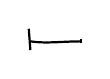
\begin{tikzpicture}[x=1cm,y=1cm,baseline=-.05cm]\draw[thick] (0,-.11)--(-.02,.16);\draw[thick] (0,0).. controls (.2,-.03) and (.4,0)..(.64,0);\draw[thick] (.64,-.025)--(.64,.025);\end{tikzpicture}}} H^{\handwritten{*}\deleted{\unsure{k|i}}}_{\mathrm{cris}}(X)
\]
